\documentclass[tikz,border=10pt]{standalone}
\usepackage[T1]{fontenc}
\usepackage{lmodern}
\usepackage{amsmath}
\renewcommand{\familydefault}{\sfdefault}
\usetikzlibrary{arrows.meta,calc}

% Vector artwork; compile with pdflatex channelmapping.tex.
\definecolor{ink}{HTML}{243447}
\definecolor{muted}{HTML}{5C6978}
\definecolor{source}{HTML}{0072B2}
\definecolor{candidate}{HTML}{B5D9EC}
\definecolor{target}{HTML}{C45126}
\definecolor{copy}{HTML}{00866A}
\definecolor{outside}{HTML}{A6ADB5}
\definecolor{rule}{HTML}{D9E0E7}
\definecolor{panel}{HTML}{F5F8FB}

\tikzset{
  source dot/.style={circle,fill=source,draw=source,minimum size=7pt,inner sep=0pt},
  candidate dot/.style={circle,fill=candidate,draw=source!55,minimum size=7pt,inner sep=0pt},
  outside dot/.style={circle,fill=outside,draw=outside,minimum size=7pt,inner sep=0pt},
  target dot/.style={rectangle,draw=target,fill=white,line width=1.1pt,minimum size=8pt,inner sep=0pt},
  flow/.style={-{Stealth[length=6pt]},draw=muted,line width=1.2pt},
  threshold/.style={draw=muted,dashed,line width=.8pt},
  heading/.style={font=\small\bfseries,align=center},
  label/.style={font=\scriptsize,align=center,text=muted}
}
\newcommand{\headoutline}{%
  \draw[line width=1pt] (0,0) ellipse (1.25 and 1.55);
  \draw[line width=1pt] (-.20,1.55) -- (0,1.88) -- (.20,1.55);
  \draw[line width=1pt] (-1.25,.18) to[out=180,in=90] (-1.48,0)
    to[out=270,in=180] (-1.25,-.18);
  \draw[line width=1pt] (1.25,.18) to[out=0,in=90] (1.48,0)
    to[out=270,in=0] (1.25,-.18);
}

\begin{document}
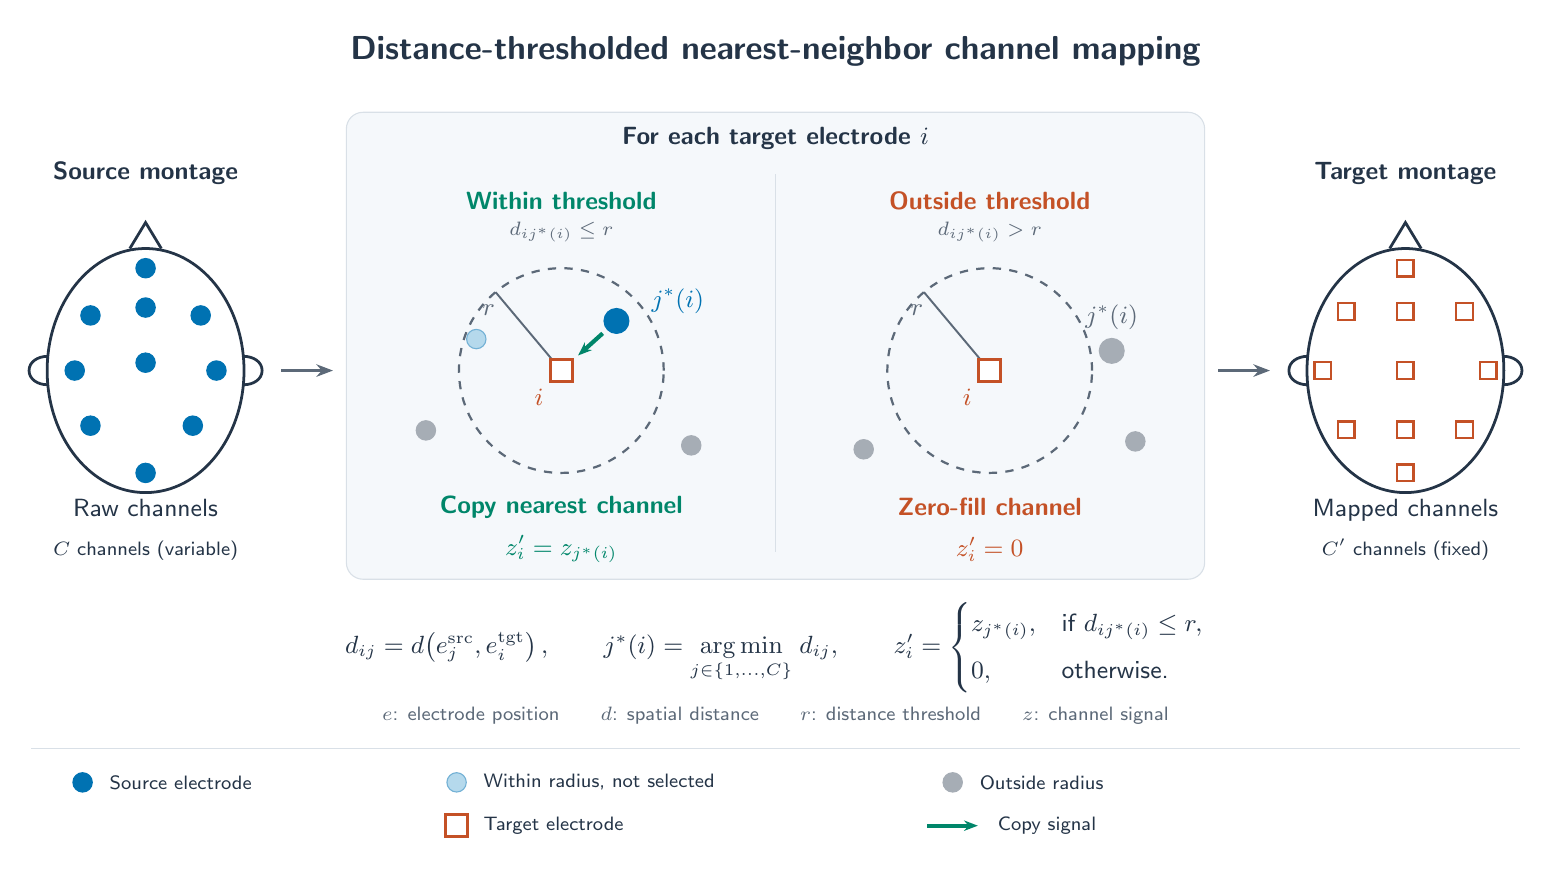
\begin{tikzpicture}[font=\sffamily, text=ink, draw=ink]
\node[font=\large\bfseries] at (0,4.05)
  {Distance-thresholded nearest-neighbor channel mapping};

% A single mapping stage with two alternative outcomes.
\filldraw[fill=panel,draw=rule,rounded corners=6pt]
  (-5.45,-2.65) rectangle (5.45,3.28);
\node[font=\small\bfseries] at (0,2.95) {For each target electrode $i$};
\draw[draw=rule] (0,-2.30) -- (0,2.50);

% Source montage: the channel count may vary across recordings.
\begin{scope}[shift={(-8,0)}]
  \node[heading] at (0,2.50) {Source montage};
  \headoutline
  \foreach \x/\y in {0/1.30,-.70/.70,0/.80,.70/.70,-.90/0,0/.10,.90/0,-.70/-.70,.60/-.70,0/-1.30}
    \node[source dot] at (\x,\y) {};
  \node[font=\small,align=center] at (0,-2.02)
    {Raw channels\\[3pt]{\scriptsize $C$ channels (variable)}};
\end{scope}
\draw[flow] (-6.28,0) -- (-5.62,0);

% Case 1: the nearest source is inside the radius; another source
% is also inside but farther away (0.94 < 1.15 < 1.30).
\begin{scope}[shift={(-2.72,0)}]
  \node[heading,text=copy] at (0,2.16) {Within threshold};
  \node[label] at (0,1.76) {$d_{i j^*(i)}\leq r$};
  \draw[threshold] (0,0) circle (1.30);
  \draw[draw=muted,line width=.7pt] (0,0) -- (-.835, .996)
    ;
  \node[font=\small,text=muted,anchor=east] at (-.72,.77) {$r$};
  \node[source dot,minimum size=9pt] (selected) at (.70,.63) {};
  \node[font=\small,text=source] at (1.48,.88) {$j^*(i)$};
  \node[candidate dot] at (-1.08,.40) {};
  \node[outside dot] at (-1.72,-.76) {};
  \node[outside dot] at (1.65,-.95) {};
  \node[target dot] (accepted) at (0,0) {};
  \node[font=\small,text=target,below left=3pt] at (accepted) {$i$};
  \draw[-{Stealth[length=5pt]},draw=copy,line width=1.5pt,shorten <=2pt,shorten >=2pt]
    (selected) -- (accepted);
  \node[font=\small\bfseries,text=copy,align=center] at (0,-2.02)
    {Copy nearest channel\\[4pt]$z'_i=z_{j^*(i)}$};
\end{scope}

% Case 2: every source lies outside the radius. The marked nearest
% source is genuinely closest (1.57 < 1.89 < 2.06).
\begin{scope}[shift={(2.72,0)}]
  \node[heading,text=target] at (0,2.16) {Outside threshold};
  \node[label] at (0,1.76) {$d_{i j^*(i)}>r$};
  \draw[threshold] (0,0) circle (1.30);
  \draw[draw=muted,line width=.7pt] (0,0) -- (-.835,.996)
    ;
  \node[font=\small,text=muted,anchor=east] at (-.72,.77) {$r$};
  \node[outside dot,minimum size=9pt] (rejected) at (1.55,.25) {};
  \node[font=\small,text=muted,above=4pt] at (rejected) {$j^*(i)$};
  \node[outside dot] at (-1.60,-1.00) {};
  \node[outside dot] at (1.85,-.90) {};
  \node[target dot] (empty) at (0,0) {};
  \node[font=\small,text=target,below left=3pt] at (empty) {$i$};
  \node[font=\small\bfseries,text=target,align=center] at (0,-2.02)
    {Zero-fill channel\\[4pt]$z'_i=0$};
\end{scope}

% Fixed target montage; square markers identify target locations,
% independently of whether their resulting channel is copied or zero-filled.
\draw[flow] (5.62,0) -- (6.28,0);
\begin{scope}[shift={(8,0)}]
  \node[heading] at (0,2.50) {Target montage};
  \headoutline
  \foreach \x/\y in {0/1.30,-.75/.75,0/.75,.75/.75,-1.05/0,0/0,1.05/0,-.75/-.75,0/-.75,.75/-.75,0/-1.30}
    \node[target dot,minimum size=6pt,line width=.9pt] at (\x,\y) {};
  \node[font=\small,align=center] at (0,-2.02)
    {Mapped channels\\[3pt]{\scriptsize $C'$ channels (fixed)}};
\end{scope}

% Consistent indexing and an explicit definition of the distance.
\node[font=\small,inner sep=10pt] at (0,-3.52) {%
  $d_{ij}=d\!\left(e_j^{\mathrm{src}},e_i^{\mathrm{tgt}}\right),
   \qquad j^*(i)=\underset{j\in\{1,\ldots,C\}}{\arg\min}\;d_{ij},
   \qquad z'_i=\begin{cases}
     z_{j^*(i)}, & \text{if } d_{i j^*(i)}\leq r,\\[4pt]
     0, & \text{otherwise.}
   \end{cases}$};
\node[label] at (0,-4.38)
  {$e$: electrode position\qquad $d$: spatial distance\qquad $r$: distance threshold\qquad $z$: channel signal};

% Compact, separate legend; no source is described as both nearest
% and unselected within the same case.
\draw[draw=rule] (-9.45,-4.80) -- (9.45,-4.80);
\node[source dot] at (-8.80,-5.23) {};
\node[font=\scriptsize,anchor=west] at (-8.58,-5.23) {Source electrode};
\node[candidate dot] at (-4.05,-5.23) {};
\node[font=\scriptsize,anchor=west] at (-3.83,-5.23) {Within radius, not selected};
\node[outside dot] at (2.25,-5.23) {};
\node[font=\scriptsize,anchor=west] at (2.47,-5.23) {Outside radius};
\node[target dot] at (-4.05,-5.78) {};
\node[font=\scriptsize,anchor=west] at (-3.83,-5.78) {Target electrode};
\draw[-{Stealth[length=5pt]},draw=copy,line width=1.5pt]
  (1.93,-5.78) -- (2.57,-5.78);
\node[font=\scriptsize,anchor=west] at (2.70,-5.78) {Copy signal};
\end{tikzpicture}
\end{document}
